 \documentclass{article}
\usepackage{cite}
\usepackage{inputenc}
\usepackage{setspace}
\usepackage[margin=0.75in]{geometry}
\usepackage[style=numeric]{biblatex}
\addbibresource{../bibs/ref.bib}
\usepackage{float}
\usepackage{graphicx}
\graphicspath{ {./images/} }


\onehalfspace
\setlength{\parindent}{0pt}
\setlength{\parskip}{1em}



\begin{document}

\begin{center}
  \LARGE{\textbf{Real-world Functional Programming}} \\
  \Large{Coursework Part I Report} \\
  \normalsize{14274056 Junsong Yang (psyjy3)} \\
  \today
\end{center}


\begin{normalsize}
  \section{Task I.1}

  \begin{figure}[H]

    \begin{minipage}[b]{0.48\linewidth}
      \centering
      \centerline{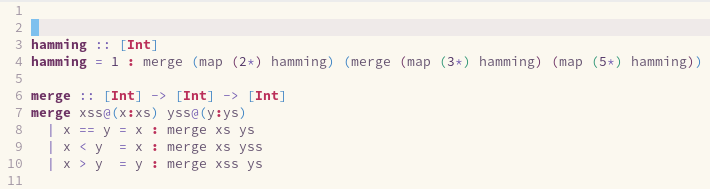
\includegraphics[width=8.0cm]{Hamming}}
      % \vspace{1.5cm}
      \centerline{ (a) Hamming Function Definition}\medskip
    \end{minipage}
    \hfill
    \begin{minipage}[b]{0.48\linewidth}
      \centering
      \centerline{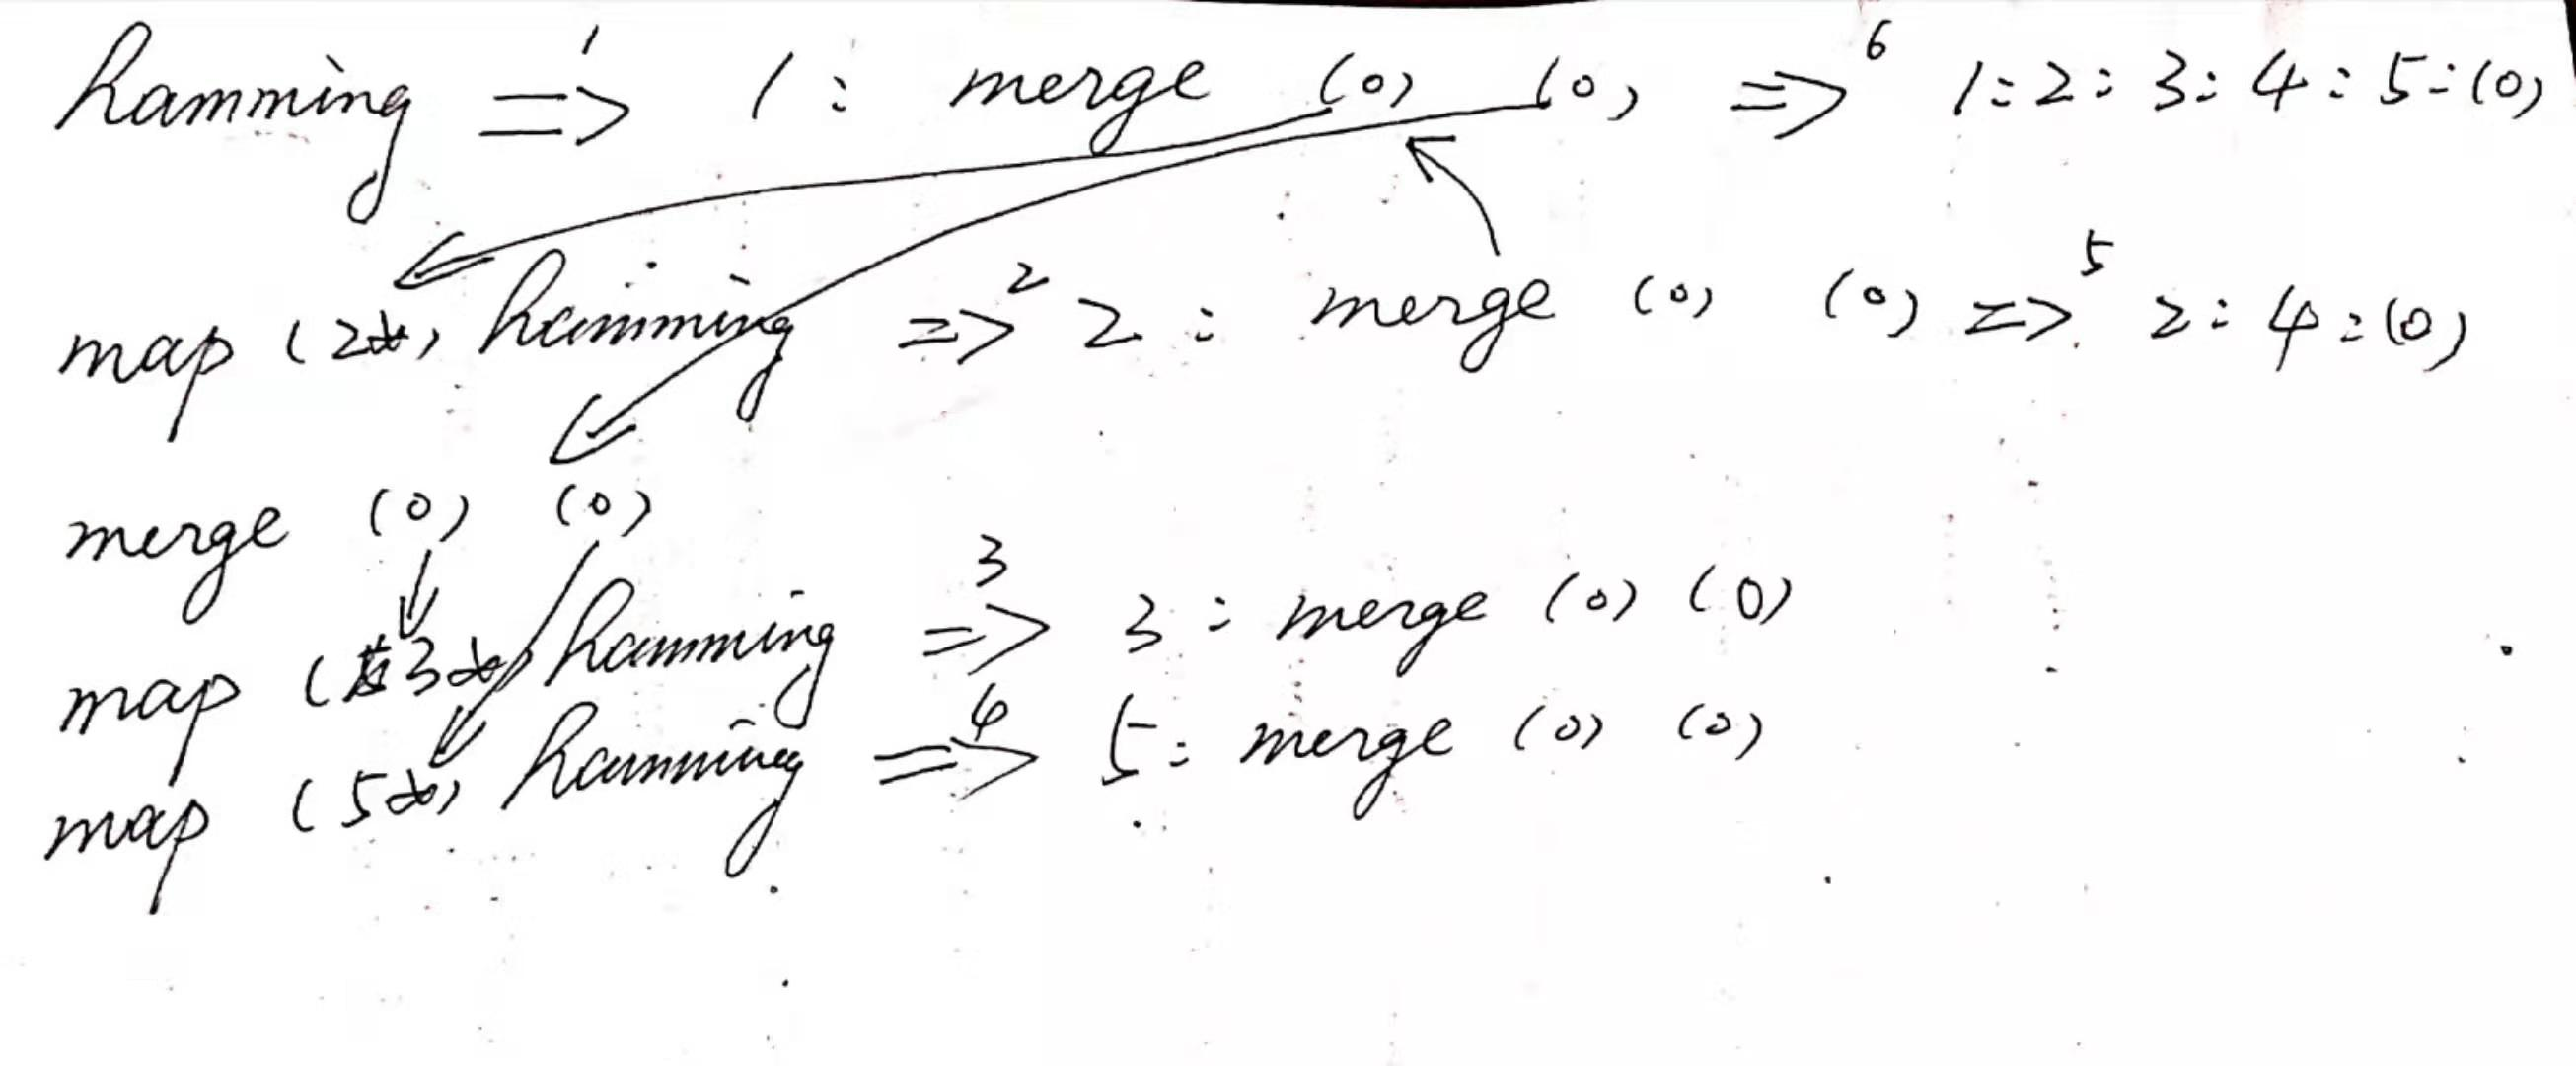
\includegraphics[width=8.0cm]{cyclic}}
      % \vspace{1.5cm}
      \centerline{ (b) Cyclic Graph}\medskip
    \end{minipage}
    % 
    \caption{TaskI.1}
    \label{fig:taskI.1}
    % 
  \end{figure}


  Hence, the hamming function can be defined as a infinite list in a recursive
  manner. As Figure \ref{fig:taskI.1} (a) shows, the type of hamming function is
  a list of Int. This implementation using map function to calculate 2x, 3x and
  5x and then merge then together as Figure \ref{fig:taskI.1} (b) demonstrated
  how it was evaluated.

  \section{Task I.2}

  \begin{figure}[H]
    \centering
    \centerline{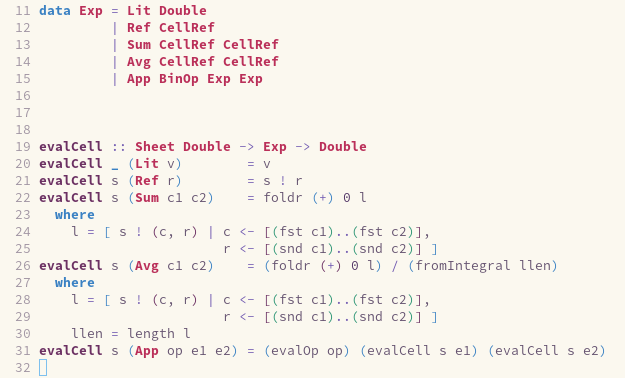
\includegraphics[scale=0.6]{Sheet}}
    \caption{Extended Evaluator}
    \label{fig:sheet}
  \end{figure}

  Figure \ref{fig:sheet} demostrates how evalCell function was extended to
  support Sum and Avg expression. The key idea of this implemetation is to given
  to CellRef c1 and c2, find every cell in between. Next, lookup corresponding
  values in the given sheet s. Then put all the values found in sheet s in list
  l. Finally using foldr to calculate the sum of all values.

  The similiar idea was used to implemetate the evaluation of Avg expression but
  a further step was taken to yield the average value.

  The most obvious weakness of this evaluator is that it will stuck in infinite
  loop when there are cyclic references in the given sheet. As the type
  signature indicates, the evalCell function will return a Double for every
  given sheet s and an Exp, which means when the Exp is Ref, it will keep
  evaluating until a Double can be returned. If there is a cyclic reference,
  this evaluator will keep evaluating without return.

  One simple solution to this problem is to maintain a seperate list to keep
  track of the evaluation of Ref Exp. This list works like stack but disallowing
  duplicated elements. A cell will of pushed to the stack if it contains Ref Exp
  as well as the reference cell. Then continue to evaluate that reference cell,
  if it returns, which means there is no cyclic reference. Hence those cell can
  be popped off the stack. If a cell that contains Ref Exp already exists in the
  stack that there must be a cyclic reference. Therefore, the evaluator can just
  return fail without continue evaluating.

  \section{Task I.3}

  In skew binary random access list, a number is represented by a sequence of
  digits starting from least significant bit to the most significant bit. Each
  digit is associated with weight predefined by the positional system.
  
  \begin{figure}[H]
    \centering
    \centerline{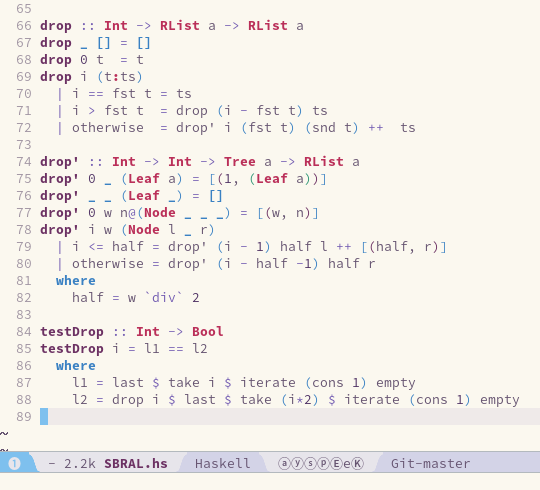
\includegraphics[scale=0.6]{SBRAL-Drop}}
    \caption{Drop Function}
    \label{fig:drop}
  \end{figure}

  Figure \ref{fig:drop} shows the implementation of drop function which drops
  the first n elements from the list. The drop function takes an integer and a
  RList as input and return a RList without the first n elments as output. If
  the tree is empty which means nothing can be dropped, hence empty list is
  returned. If the input integer is zero which means nothing needs to be
  dropped, then the same list taken as input will be returned. If the size of
  the first element in the list is equals to the number of elements need to be
  dropped, then the tail of the input list will be returned. If the number of
  elements need to be dropped is greater that the size of first element in the
  list, then the first element will be dropped and the drop function will be
  called recursively to continue processing the remaining list. The operations
  mentioned above would run id constant time.

  The next case of the drop function determines the overall time complexity. If
  the number of elements need to be dropped is less than the size of first
  element in the list, then a helper function drop' will be called. The drop'
  function takes two integers and a tree as input and returns a RList. Similar
  to the first two cases of drop function, the first three cases of drop'
  function are practically doing nothing. Since the input tree is complete
  binary leaf tree, the size of tree will be halved for every
  element dropped from the tree. Therefore, the overall time complexity is $O
  (log{}n)$. If the number of elements need to be dropped is 
  less than or equals to the half size of the input tree, then only the left
  chilren of the input tree will be processed. Otherwise, the left children will
  be dropped and the right children will be processed accordingly. The drop'
  function will be called recursively untill the drop is finished or there
  nothing to drop and return the final result.

  A test function called testDrop id created to test the drop function. The key
  idea is the RList which represents n should equal to the RList that represents
  2n without the first n elements.

  \section{Task I.4}
  
  \begin{figure}[H]
    \centering
    \centerline{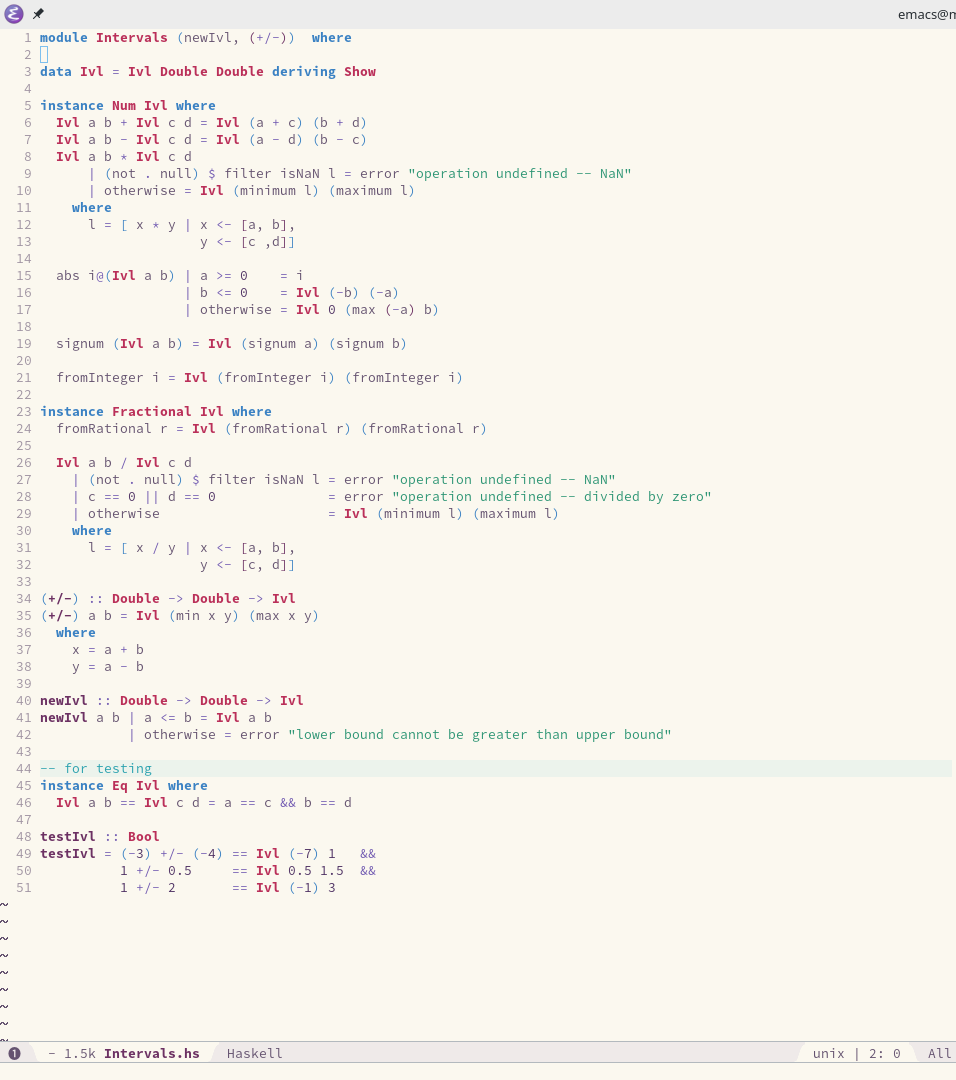
\includegraphics[scale=0.4]{Intervals}}
    \caption{Intervals}
    \label{fig:intervals}
  \end{figure}
  
  Figure \ref{fig:intervals} shows how Ivl was made an instance of Num and
  Fractional class. As an instance of Num class, (+), (-) and abs functions were
  implemetated according the rule of interval arithmetic.

  As for (*) function, there are a few cases that NaN may be yield which means
  the arithmetic operation is illegal. Hence, the (*) function will return error
  every time NaN occurs. The signum function takes an Ivl as input and return an
  Ivl with the signum value of lower bound and signum value of upper bound. the
  fromIntegral function takes an int as input and returns an Ivl with the same
  value converted from input.

  the fromRational function in Fractional class works in a similar way as the
  fromIntegral function. The (/) function also employed the same manner to deal
  with NaN. Furthermore, in this implementation, divided by zero is not allowed.
  Hence, if divided by zero ever occurs, an error will be returned.

  As for the (+/-) function, the key idea is to calculate the symmetric interval
  around a specific number. The input numbers may be negative, to deal with this
  situation, the lower bound of the resulting Ivl is the smaller value of the
  result of plus and minus of the two input value while the upper bound is the
  larger value of the result of plus and minus of the two input values. A few
  test cases is provided in the testIvl function to test the result of the (+/-)
  function. 

  \section{Task I.5}

  \begin{figure}[H]

    \begin{minipage}[b]{0.48\linewidth}
      \centering
      \centerline{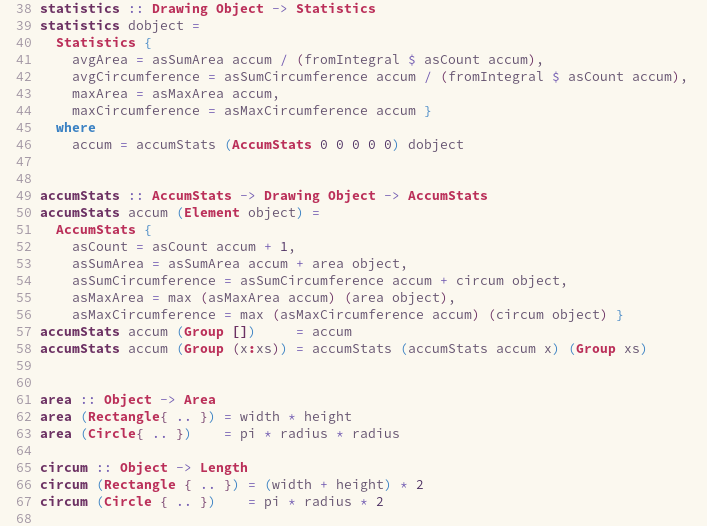
\includegraphics[width=8.0cm]{Stats}}
      % \vspace{1.5cm}
      \centerline{ (a) Recursive Statistics}\medskip
    \end{minipage}
    \hfill
    \begin{minipage}[b]{0.48\linewidth}
      \centering
      \centerline{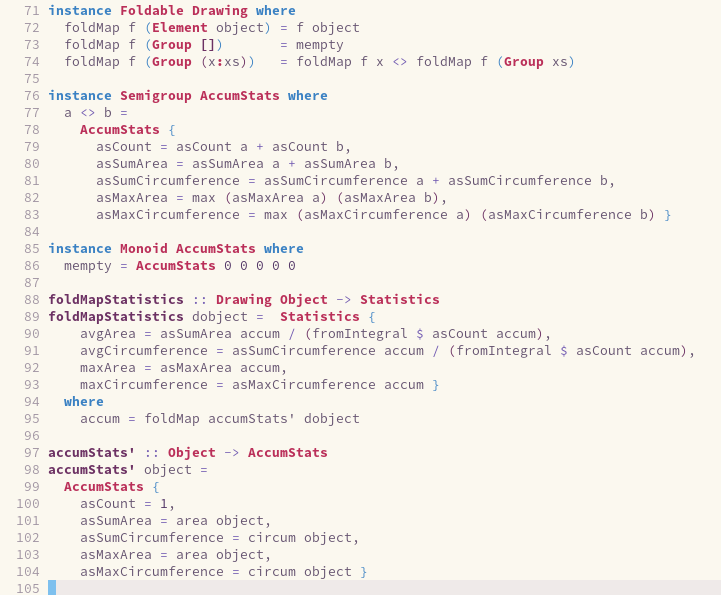
\includegraphics[width=8.0cm]{StatsFoldMap}}
      % \vspace{1.5cm}
      \centerline{ (b) Statistics using foldMap}\medskip
    \end{minipage}
    % 
    \caption{TaskI.5 1 2}
    \label{fig:taskI.5.1.2}
    % 
  \end{figure}

  Figure \ref{fig:taskI.5.1.2} shows how the statistics functions were
  implemetated using two different approach.


  \begin{figure}[H]

    \begin{minipage}[b]{0.48\linewidth}
      \centering
      \centerline{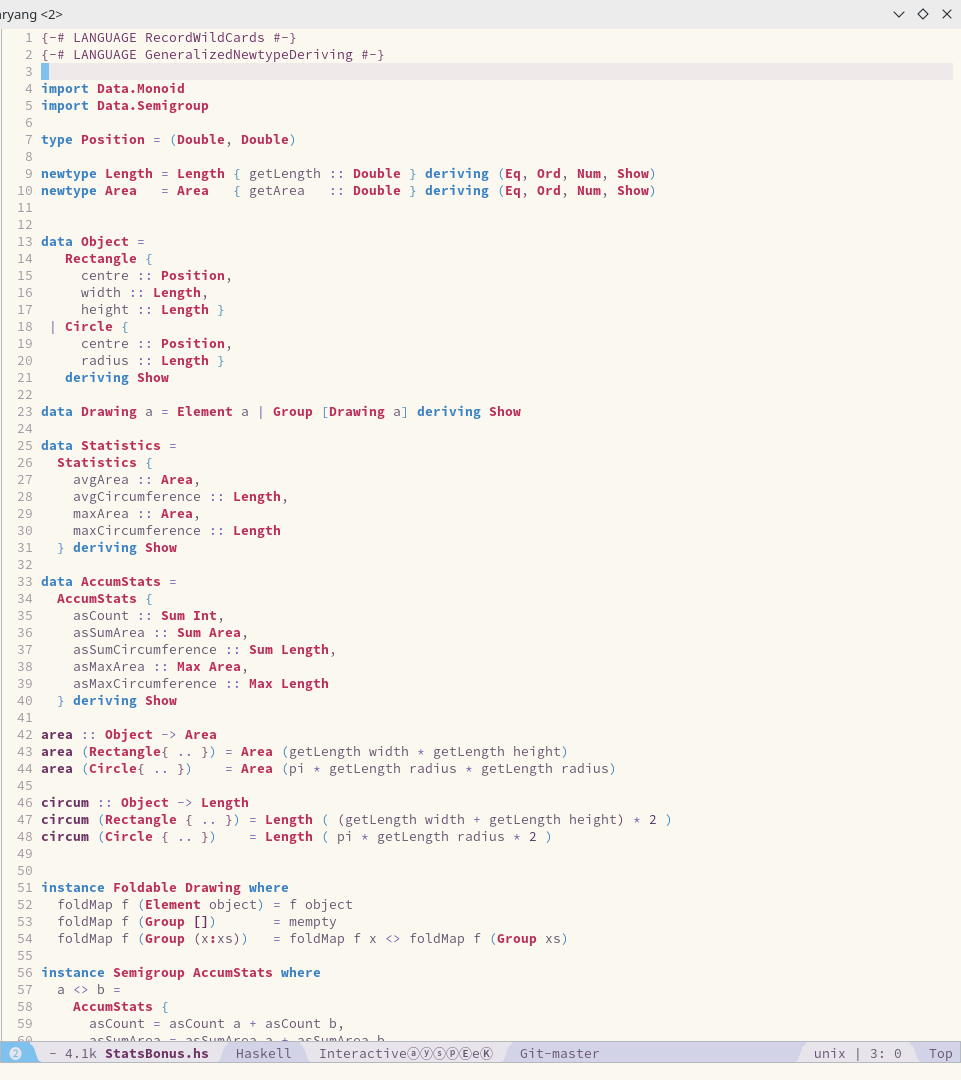
\includegraphics[width=8.0cm]{StatsBonus}}
      % \vspace{1.5cm}
      \centerline{ (a) Recursive Statistics for newtype}\medskip
    \end{minipage}
    \hfill
    \begin{minipage}[b]{0.48\linewidth}
      \centering
      \centerline{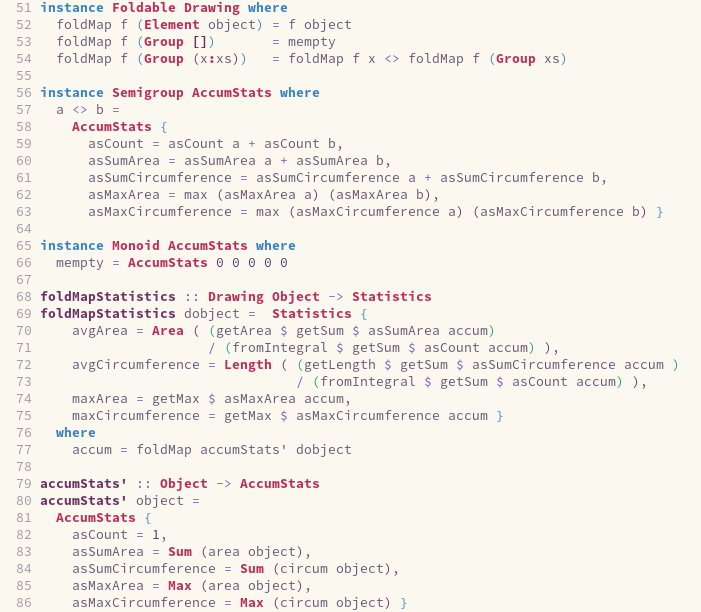
\includegraphics[width=8.0cm]{StatsBonusFoldMap}}
      % \vspace{1.5cm}
      \centerline{ (b) Statistics using foldMap for newtype}\medskip
    \end{minipage}
    % 
    \caption{TaskI.5 3}
    \label{fig:taskI.5.3}
    % 
  \end{figure}

  


\end{document}


